\tikzset{every picture/.style={line width=0.75pt}} %set default line width to 0.75pt        

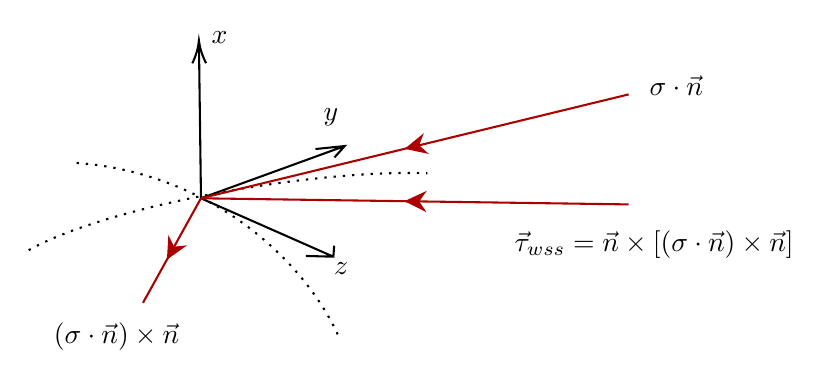
\begin{tikzpicture}[x=0.75pt,y=0.75pt,yscale=-1,xscale=1]
%uncomment if require: \path (0,233); %set diagram left start at 0, and has height of 233
%Shape: Axis 2D [id:dp1284680579045342] 
\draw  (262.36,123.1) -- (326.14,151.24)(331.61,97.93) -- (262.36,123.1) -- cycle (326.53,145.95) -- (326.14,151.24) -- (312.95,150.88) (317.53,99.37) -- (331.61,97.93) -- (326.68,103.41)  ;
%Straight Lines [id:da6599545564220138] 
\draw [color={rgb, 255:red, 0; green, 0; blue, 0 }  ,draw opacity=1 ][line width=0.75]    (262.37,123.1) -- (261.39,49.1) ;
\draw [shift={(261.37,47.1)}, rotate= 89.25] [color={rgb, 255:red, 0; green, 0; blue, 0 }  ,draw opacity=1 ][line width=0.75]    (10.93,-3.29) .. controls (6.95,-1.4) and (3.31,-0.3) .. (0,0) .. controls (3.31,0.3) and (6.95,1.4) .. (10.93,3.29)   ;
%Curve Lines [id:da612751287350806] 
\draw  [dash pattern={on 0.84pt off 2.51pt}]  (179.37,148.1) .. controls (216.42,127.05) and (315.42,109.05) .. (371.42,111.05) ;
%Curve Lines [id:da7220443498017698] 
\draw  [dash pattern={on 0.84pt off 2.51pt}]  (202.42,106.05) .. controls (268.47,111) and (312.42,154.05) .. (328.42,189.05) ;
%Straight Lines [id:da9447558643950482] 
\draw [color={rgb, 255:red, 170; green, 0; blue,0}, draw opacity=1 ][line width=0.75]    (468.42,73.05) -- (262.37,123.1) ;
\draw [shift={(360.53,99.26)}, rotate= 346.35] [fill={rgb, 255:red, 170; green, 0; blue, 0 }  ,fill opacity=1 ][line width=0.08]  [draw opacity=0] (10.72,-5.15) -- (0,0) -- (10.72,5.15) -- (7.12,0) -- cycle;
%Straight Lines [id:da5334420450686234] 
\draw [color={rgb, 255:red, 170; green, 0; blue,0}, draw opacity=1 ][line width=0.75]    (468.42,126.05) -- (262.37,123.1) ;
\draw [shift={(360.39,124.5)}, rotate= 0.82] [fill={rgb, 255:red, 170; green, 0; blue, 0 }  ,fill opacity=1 ][line width=0.08]  [draw opacity=0] (10.72,-5.15) -- (0,0) -- (10.72,5.15) -- (7.12,0) -- cycle;
%Straight Lines [id:da07191031048171115] 
\draw [color={rgb, 255:red, 170; green, 0; blue,0}, draw opacity=1 ][line width=0.75]    (262.36,123.1) -- (234.42,173.47) ;
\draw [shift={(245.96,152.65)}, rotate= 299.02] [fill={rgb, 255:red, 170; green, 0; blue, 0 }  ,fill opacity=1 ][line width=0.08]  [draw opacity=0] (10.72,-5.15) -- (0,0) -- (10.72,5.15) -- (7.12,0) -- cycle;
% Text Node
\draw (266,41.4) node [anchor=north west][inner sep=0.75pt]    {$x$};
% Text Node
\draw (320,78.4) node [anchor=north west][inner sep=0.75pt]    {$y$};
% Text Node
\draw (325,152.4) node [anchor=north west][inner sep=0.75pt]    {$z$};
% Text Node
\draw (477,62.4) node [anchor=north west][inner sep=0.75pt]    {$\sigma \cdot \vec{n}$};
% Text Node
\draw (190,181.4) node [anchor=north west][inner sep=0.75pt]    {$( \sigma \cdot \vec{n})\times \vec{n}$};
% Text Node
\draw (412,137.4) node [anchor=north west][inner sep=0.75pt]    {$\vec{\tau}_{wss}=\vec{n}\times\left[(\sigma\cdot\vec{n})\times \vec{n}\right]$};


\end{tikzpicture}
